The first test is devoted to investigating the distribution of the velocities of the particles after sufficiently long time. From statistical mechanics, we know that the velocities of a $2$-dimensional gas at equilibrium will distribute according to Maxwell's velocity distribution: 
\[
	p(v) = \frac{mv}{k_B T} \exp{\left(- \frac{mv^2}{2 k_B T}\right)},
\]
where $k_B$ is Boltzmann's constant, $T$ the absolute temperature, and $m$ the mass of the particles. It is essential that the all the particles have the same mass $m$, as will become apparent in the following section [LINK].

We initialise an ensemble of particles with velocities $\mathbf{v} = [v_0 \cos{\theta} , v_0 \sin{\theta}]$ with $\theta \sim \U[0,2\pi]$. The initial distribution of the velocities is therefore $C\delta (v - v_0)$. After simulating sufficiently long, the distribution is as shown in figure \ref{fig:dist_1}.

\begin{figure}[htb]
	\label{fig:dist_1}
	\centering
	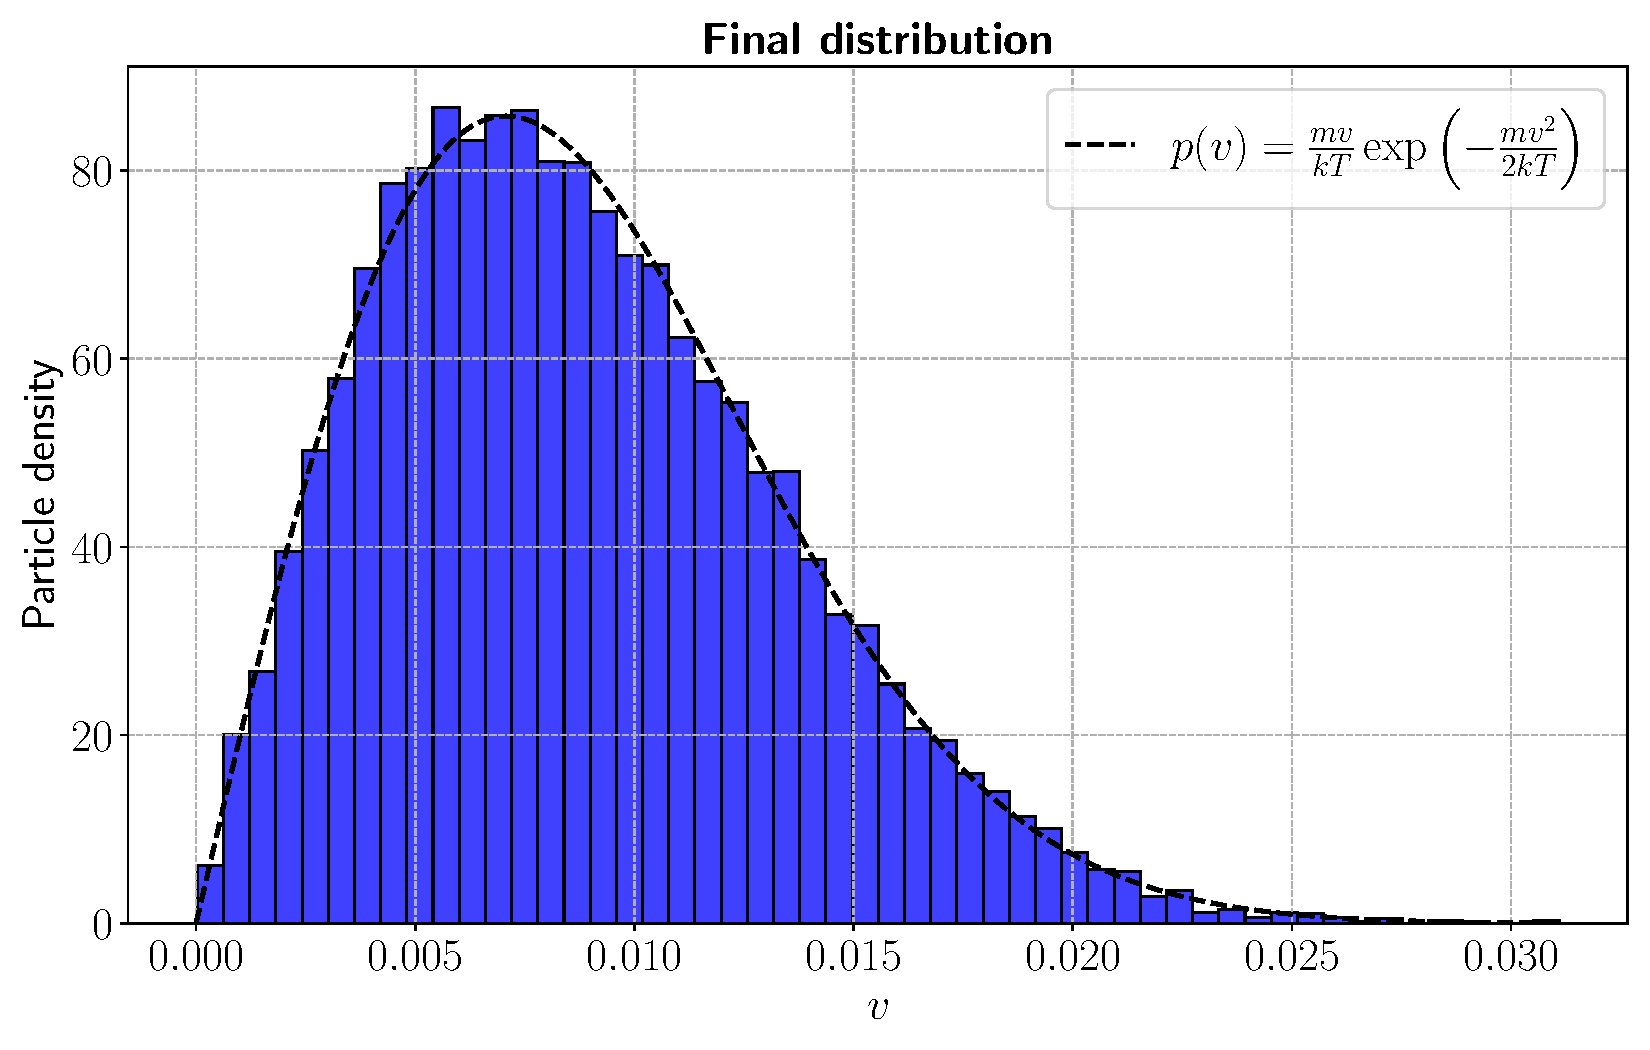
\includegraphics[width=\textwidth]{../fig/dist_1}
	\caption{Distribution of velocities in an ensemble of $10000$ particles after $200 \,\text{s}$.}
\end{figure}